\documentclass[]{scrartcl}
\usepackage{graphicx}
\usepackage{geometry}
\geometry{
	a4paper,
	total={170mm,257mm},
	left=20mm,
	top=20mm,
}


%opening
\title{SDD -Client Low Level Design}
\author{Brandon Smith, Nieka Gutenberger, Joseph Coppin, Ryan Frazier, Trevor Jewkes}

\begin{document}

\maketitle

\centerline{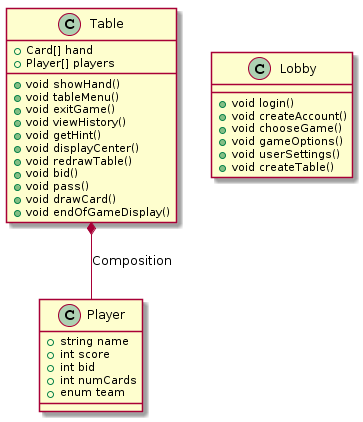
\includegraphics{Client_Class_diagram.png}}
\centerline{Client Class Diagram}

\section{Table}

\subsection{Card[] hand}
	An array of cards holding each players hand.
\subsection{Player[] players}
	An array of player objects.
\subsection{void showHand()}
	A function that prints out the player’s hand onto the GUI.
\subsection{void tableMenu()}
	A menu dropdown that includes the following: (plus any other options we see fit to add in the future)
	\subsubsection{void exitGame()}
		Facilitates a call to the server about early game withdrawal.
	\subsubsection{void viewHistory()}
		Shows a history of each trick in the given round
	\subsubsection{void getHint()}
		Provides the user with a “good” playable card. (Possibly using the logic from the hard AI)
\subsection{void displayCenter()}
	Controls the display of the center play area as the game is played.
\subsection{void redrawTable()}
	Updates the table after each move is made, in between tricks, and after each round.
\subsection{void bid()}
	Used in Spades to handle the bid scenario.
\subsection{void pass()}
	Used in Hearts to handle the pass scenario
\subsection{void drawCard()}
	Used in Crazy 8s to handle the draw card scenario.
\subsection{void endOfGameDisplay)}
	Is called at the end of a game to display winners, everyone’s final scores, and an option to play again or return to the main menu.


\section{Player}

\subsection{string name}
	String that holds the name of a player.
\subsection{int score}
	Int that holds the score of a player.
\subsection{int bid}
	Int that holds the value bidded in a game of Spades.
\subsection{int numCards}
	Int that holds the number of cards player has left to play.
\subsection{enum team}
	Marks player as in team 1, team 2 or on no team depending on game played.


\section{Lobby}
\subsection{void login()}
	This function allows for the user to enter their credentials and will send a login request to the server. 
\subsection{void createAccount()}
	This function allows for the user to create an account and send that information to the server
\subsection{void chooseGame()}
	This function will take the user's request to start one of the games and send the corresponding request to the server.
\subsection{void gameOptions()}
	This function will take the user's request to play a public or private game.
\subsection{void userSetting()}
	This function will open the window for the user to see their stats and a set amount of options.
\subsection{void createTable()}
	This function will be called to start the game and will create the table for play to begin. It will also send a start game request to the server.


\end{document}
